\section{Improvements} \label{approach}
Two new insights were leveraged to improve the fuzzing energy distribution strategy in a principled way. The improvements contain two aspects: (1) improvement of directing fuzzing toward promising regions that are more likely to have vulnerabilities; and (2) improvement of scheduling of the distribution ratio of different mutation operators.  Finally,  these improvements are organically integrated and implemented into a new tool.

%\subsection{Improvement of balance to time-consuming paths}
%As shown in insight 1, existing energy assignment formulas discriminate against time-consuming procedures. More specific, the AFL(including AFLFast)  will prefer time-saving test case and assign the basis energy based on execute time as Table \ref{EnergyBasis}. The strategy of AFLFast prefer low frequence path and spend more energy on low frequence path, this measure has effect on reduce the discrimination on TC path, but it will lead to strut on TC path sometime, and the basis energy calculation is same as AFL. We try to balance  fairness for TC path with the execute speed of fuzzers. So we change the basis energy calculation using with a specific probilities.  We will using Rule listed in Table \ref{EnergyBasis} with 70\% probilities, and using Rule listed in Table 2 with 30\%.
%
%\begin{table}[hbpt]
%\centering
%\label{EnergyBasis2}
%\caption{Basis Energy Determine Rule2}
%\begin{tabular}{|l|}
%\hline
%q $\rightarrow$ exec\_us * 0.10      $>$  avg\_exec\_us    $\rightarrow$  perf\_score = 300; \\
%q $\rightarrow$ exec\_us * 0.25      $>$  avg\_exec\_us    $\rightarrow$  perf\_score = 200;\\
%q $\rightarrow$ exec\_us * 0.50      $>$  avg\_exec\_us    $\rightarrow$  perf\_score = 150;\\
%q $\rightarrow$ exec\_us * 0.75      $>$  avg\_exec\_us    $\rightarrow$  perf\_score = 75;\\
%q $\rightarrow$ exec\_us * 2.00      $<$  avg\_exec\_us    $\rightarrow$  perf\_score = 50;\\
%q $\rightarrow$ exec\_us * 3.00      $<$  avg\_exec\_us    $\rightarrow$  perf\_score = 25;\\
%q $\rightarrow$ exec\_us * 4.00      $<$  avg\_exec\_us    $\rightarrow$  perf\_score = 10;\\
%\hline
%\end{tabular}
%\end{table}
% 
%
%And at early stage, we follow the energy assignment of original AFL, and when the path growth become flat, we prefer to make the time-consuming test case as favorable, and spend more energy. 

\subsection{Improvement of Directing Toward Promising Regions}
Inspired by AFLGo, which directs fuzzing to reach some specific code lines. We improve the guidance of AFL toward promising vulnerable code regions. The core idea is to extract semantic metrics of basic blocks of target program using light-weight Intermediate representation (IR) level static analysis. Then we instrument these qualitative weights into original program through compiler-time instrumentation. At run-time, path reward (i.e., sum of weight) is traced. If a test case is interesting, we assign energy based on its path reward. The seeds who win more rewards will be assigned with more energy. In this way, based on specific semantic metrics of code region, fuzzing could be directed to stress fuzzing those promising vulnerable regions, like sensitive regions, complex regions, deep region and rare-reach regions. 

We demonstrate an Intuitive example to explain energy assignment using the abstract control flow graph (CFG) shown in Fig.\ref{cfg}. 

\begin{figure}[t]
\centering
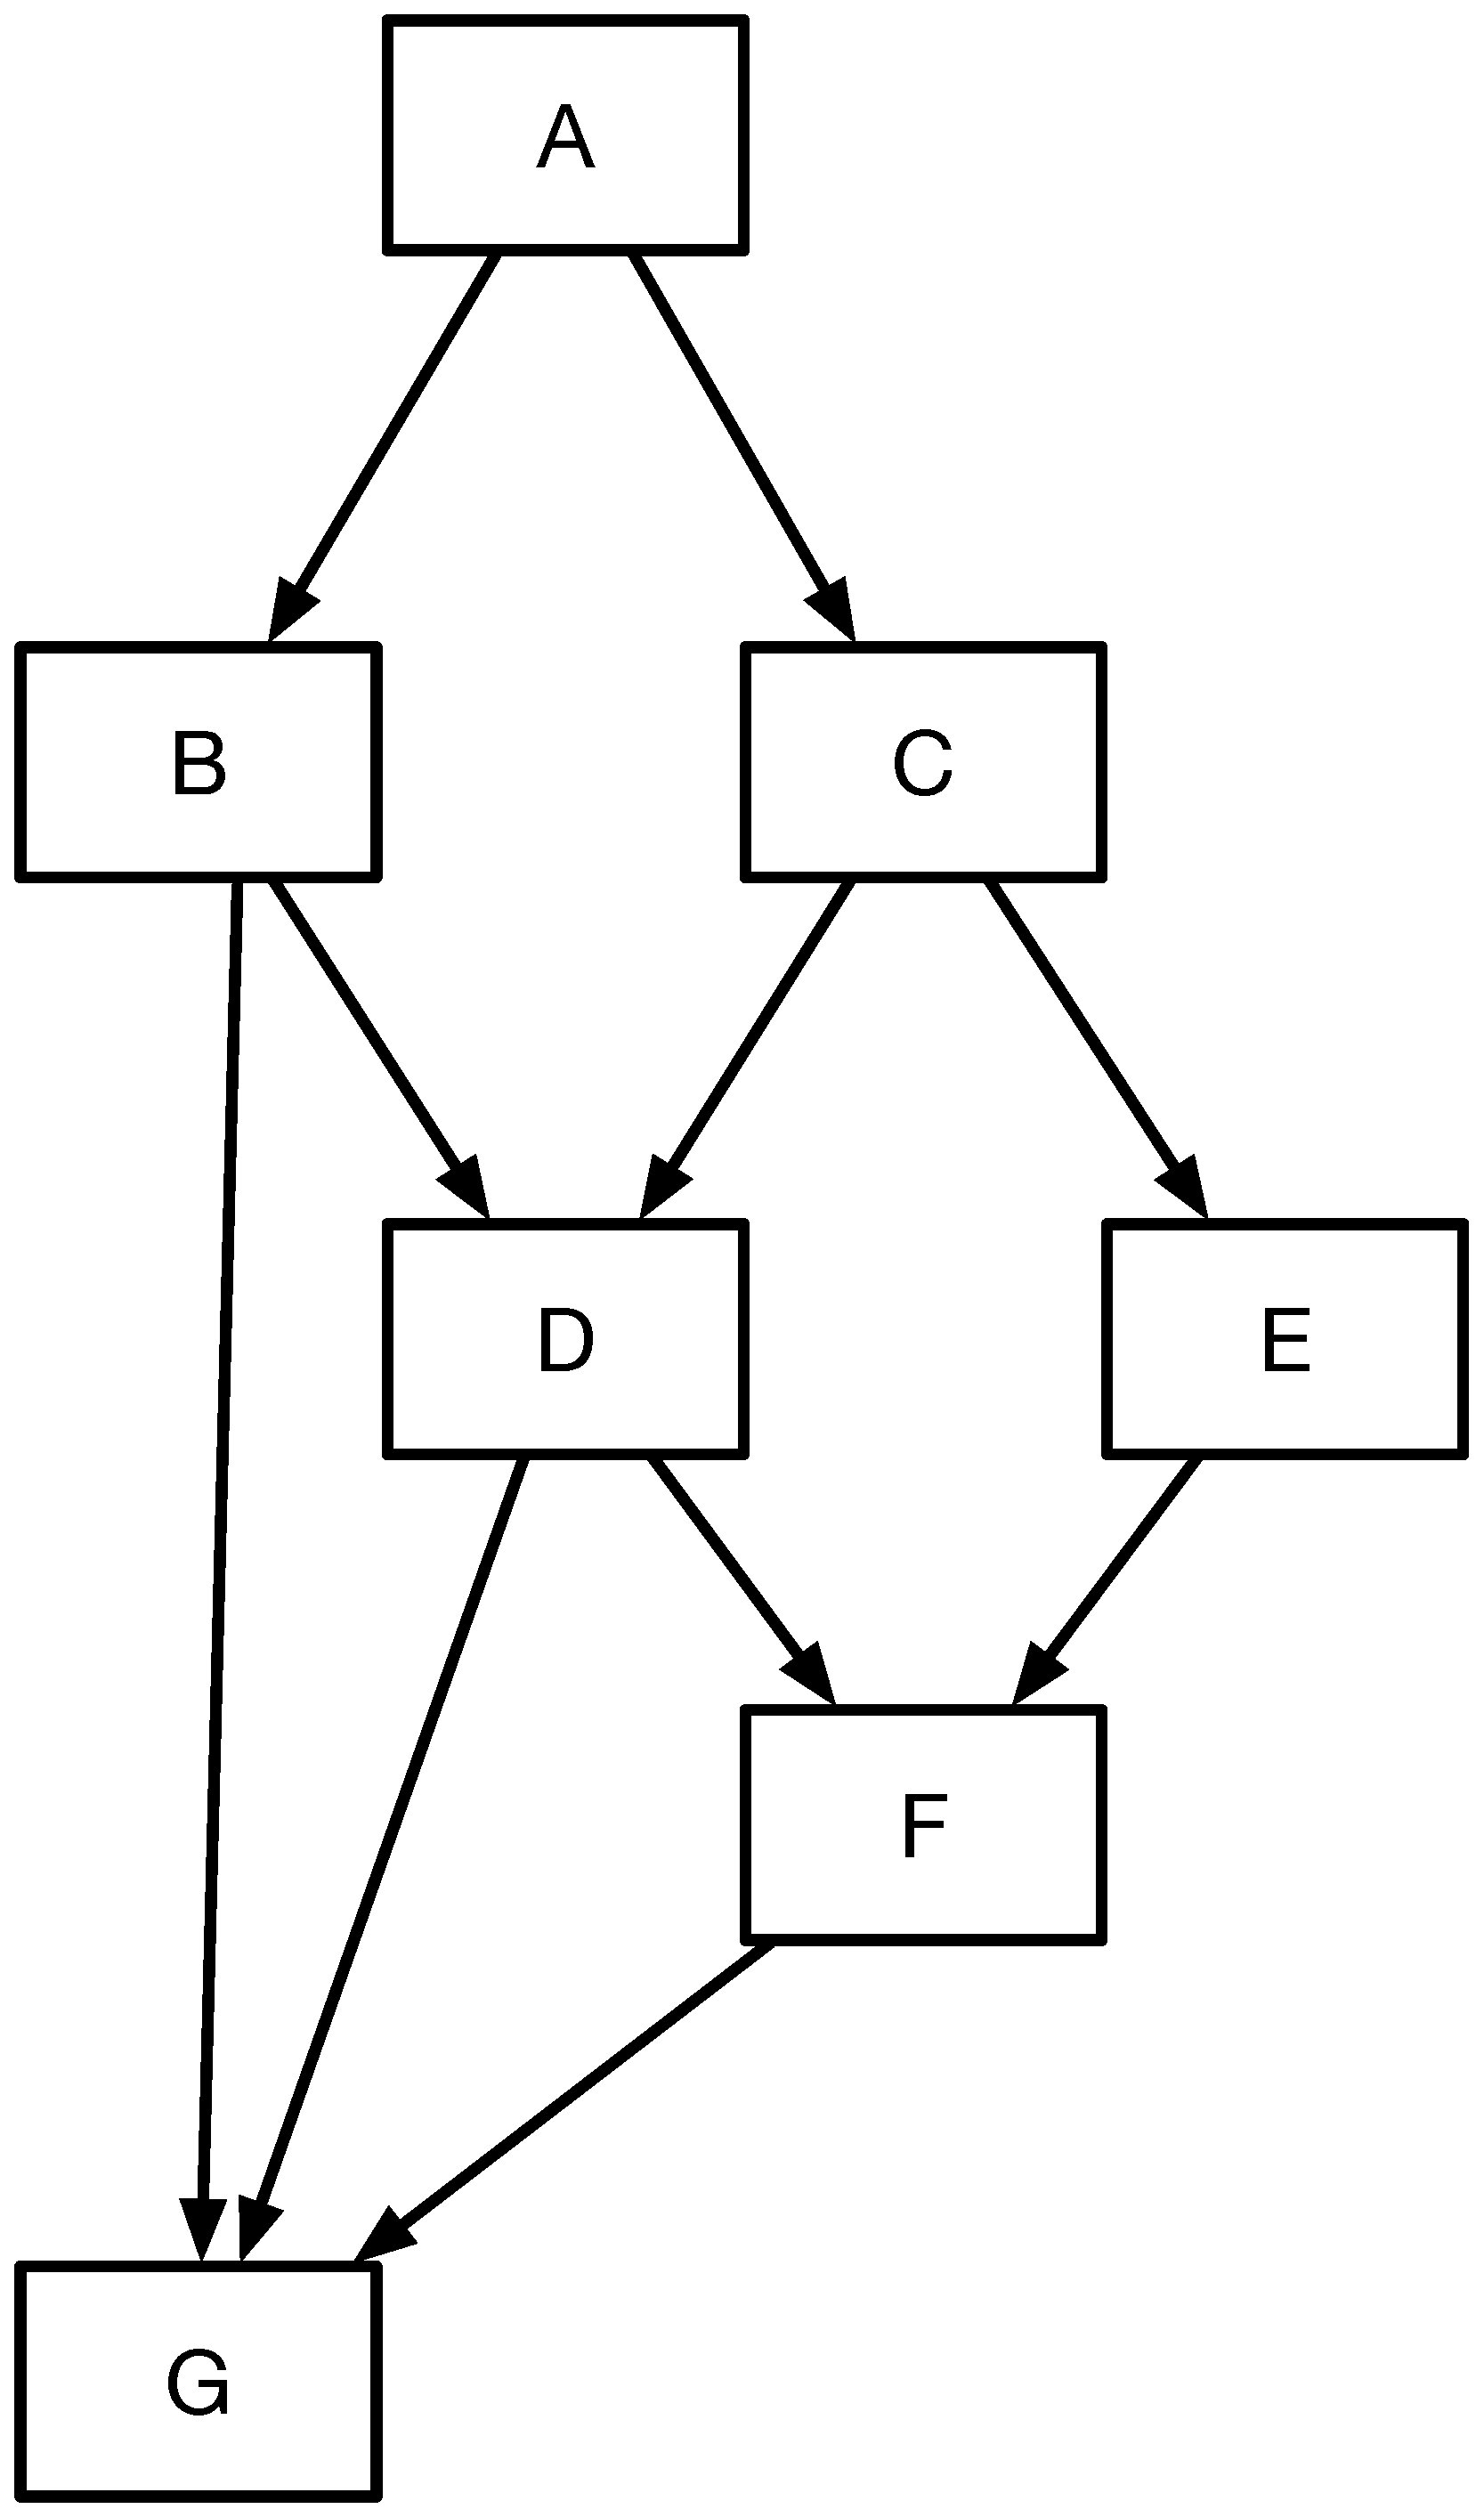
\includegraphics[width=1in]{pic/AbstractCFG.eps}
\caption{Abstract CFG}
\label{cfg}
\end{figure}

Let weight of a basic block $BB$ for a specific $metric$ be $weight_{metric}(BB)$. Then, reward of a path that executed with input $t$ could be denoted as:
\begin{equation}
Reward(t)=  \frac{\sum_{i=0}^{n} weight(BB_{i})}{n}, BB_{i} \in path(t)
\end{equation}

Sum of block weights in path $path(t)$ exercised by the input $t$ is counted. Note that we count the basic blocks in loop for multiple times. Intuitively, if test case $t$ executes the path of $p= A \rightarrow B \rightarrow D \rightarrow G$, then $Reward(t)$=$(weight_{metric}(A)$ + $weight_{metric}(B)$ + $weight_{metric}(D)$ + $weight_{metric}(G) )/4$. After an execution is finished,  the maximum, minimum reward and average reward are updated. Average reward $AvgReward$ is calculated using equation as shown below:
\begin{equation}
 AvgReward = \dfrac{MaxReward + MinReward} {2}
 \end{equation}
 
Furthermore, $Factor$ used for energy assignment is computed based on a seed's reward and average reward value. 
 \begin{equation}
Factor(t)= \dfrac{Reward(t)}{AvgReward}
 \end{equation}

$Factor$ affects the amount of energy assignment. The bigger the $Factor$ is, the more energy is assigned.  More specifically, an exponential energy assignment formula in the following is used to assign energy based on the $Factor$. Let $P_{afl}(t)$ be the energy assigned by AFL for input $t$, and energy $P(t)$ for test case $t$ assigned after improvement could be donated as following:
\begin{equation}
P(t) = P_{afl}(t) * 2^{ 10 * Factor(t)}
\end{equation}

Thus, based on institutions that the more sensitive, complex, deeper and more rarely reachable regions, the more chance to be vulnerable. Four kinds of related semantic metric are designed and used to drive fuzzing. The four kinds of semantic metric represents four kinds of promising vulnerable regions. They are sensitive region,  complex region, deep region, and rarer-reach region. Note that our metrics are one possible representation of four kinds of regions, the four regions could also be represented using other metrics.

\subsubsection{Towards Sensitive Region}
According to the intuition that if a path contains more sensitive operators like memory and string related instruments, it is more likely to occur memory corruption vulnerabilities.  Thus, a sensitive metric is designed to measure the sensitive degree of the code region (i.e., basic block). More specifically, measurement of sensitive metric is defined as follows:
\begin{equation}
SensitiveDegree(BB) =MemoryOP + StringOP
\end{equation}

Where, $SensitiveDegree$ represents the total numbers of memory and string related instruments in the basic block $BB$. 

\subsubsection{Toward Complexity Region}
Based on intuition that more complex areas are more likely to have vulnerabilities, complexity metric are designed to measure complexity of each basic block. The number of total instruments in a basic block is a simple and direct indicator to show the complexity of a code region. Thus, we used instrument number as the complex metric, and the measurement is as follows:
\begin{equation}
ComplexityDegree(BB) ={InstNum}
\end{equation}

where $ComplexityDegree$ represents the total numbers of instruments in basic block $BB$. 


\subsubsection{Toward Deep Region}

Based on intuition that it has more chance to detect vulnerability by exploring the deep path,  we define depth metric to show the deep degree of a path. It represents the distance from the function's entry block to the basic block itself. More specifically, the measurement of depth metric of basic block $BB$ as follows:

For a given basic block $BB$, all the paths $P$ that from entry block $E$ within function to the basic block $B$ are traversed, which is donated by $P=path(E,BB)$. Assume the depth of path $p_{i} \in P$ is $d_{i}$, then depth of $BB$ is as follows equation:
\begin{equation}
Depth(BB)= \dfrac{1}{ \sum_{p_{i} \in P}  \dfrac{1}{d_{i}}}
\end{equation}

Intuitively,  take Fig. \ref{cfg} as an example, to calculate depth of basic block $G$, the abstract CFG is traversed using deep first search (DFS) algorithm. And paths from entry block $A$ to $G$ are obtained firstly. They are $p_{1}=A\rightarrow B\rightarrow G$, $p_{2}=A\rightarrow B\rightarrow D\rightarrow G$,  $p_{3}=A\rightarrow C\rightarrow D\rightarrow G$, $p_{4}=A\rightarrow B\rightarrow D\rightarrow F \rightarrow G$, $p_{5}=A\rightarrow C\rightarrow D\rightarrow F \rightarrow G$, $p_{5}=A\rightarrow C\rightarrow E\rightarrow F \rightarrow G$.  The length of above paths are 2, 3, 3, 4, 4. ( i.e. $l_{p_{1}} = 2$, $l_{p_{2}}=3$, $l_{p_{3}}=3$, $l_{p_{4}}=4$ , $l_{p_{5}}=4$). Then, depth of basic block $G$ is computed as equation (7), and result is $1/(1/2 + 1/3 + 1/3 + 1/4 + 1/4) = 3/5$. Note that computation of depth is based on intra-procedure static analysis without considering function-level distance. It may sacrifice certain accuracy for conveniences of usage.

\subsubsection{Toward Rare-Reach Region}

Based on intuition that if a code region has lower reachable probability, the region may have higher chance to have issues. The reason behind this intuition is that rare-reach areas are usually not suffering from sufficient testing, especially in integration testing phase. Thus, metric called $RareReachDegree$ is defined to represent the rarely reachable degree of a region (i.e., basic block of program). More specifically, measurement of rarely reachable degree is calculated as follows.

For a given basic block $BB$, the probability to all its outgoing edges are assumed to be equal. Hence, if $succ(BB)$ denotes number of all successor basic blocks of $BB$, then $\forall b \in succ(BB)$, $TPro(B, b)$ = 1 / $succ(B).size$, where $succ(B).size > 0$.  All paths $P$ that from entry block $E$ of function to basic block $BB$ itself are traversed, and denoted by $P=path(E, BB)$.

Given a path $p_{i} \in P$, the reachable probability of $BB$ in path $p_{i}$ is calculated using below equation:
\begin{equation}
RPro(BB,p_{i})=\dfrac{1}{\prod_{j=0}^{p_{i}.size -1} TPro(B_{j}, B_{j+1})} 
\end{equation}

Furthermore, we will calculate all paths and finally get the rarely reachable degree of basic block $BB$ as follows:
\begin{equation}
RareDegree(BB)= \dfrac{1}{ \sum_{i=0}^{P.size - 1} RPro(BB, p_{i})}
\end{equation}

Similarly, take Fig.4 as an example for sake of clarity. In order to compute depth of basic block $G$, we will traverse the control flow graph using DFS algorithm and get all the paths from entry block $A$ to basic block $D$. They are $p_{1}=A\rightarrow B\rightarrow D$, $p_{2}=A\rightarrow C\rightarrow D$.  Then,  rare-reach degree of $B$ is calculated using equation (8) and (9), and the result is $1/(1* 1/2 + 1 *1/2) = 4$. 


\subsection{Improvement of Schedule of Mutators}
Existing energy assignment strategies only consider number of mutations. But they do not take into account the distribution of different granularity mutation operations in assignment number. In order to add flexible granularity-aware scheduling for different kinds of mutation operations, an understanding of different granularity mutation operators' abilities to promote path growth is needed firstly.

\begin{figure}[t]
    \centering
    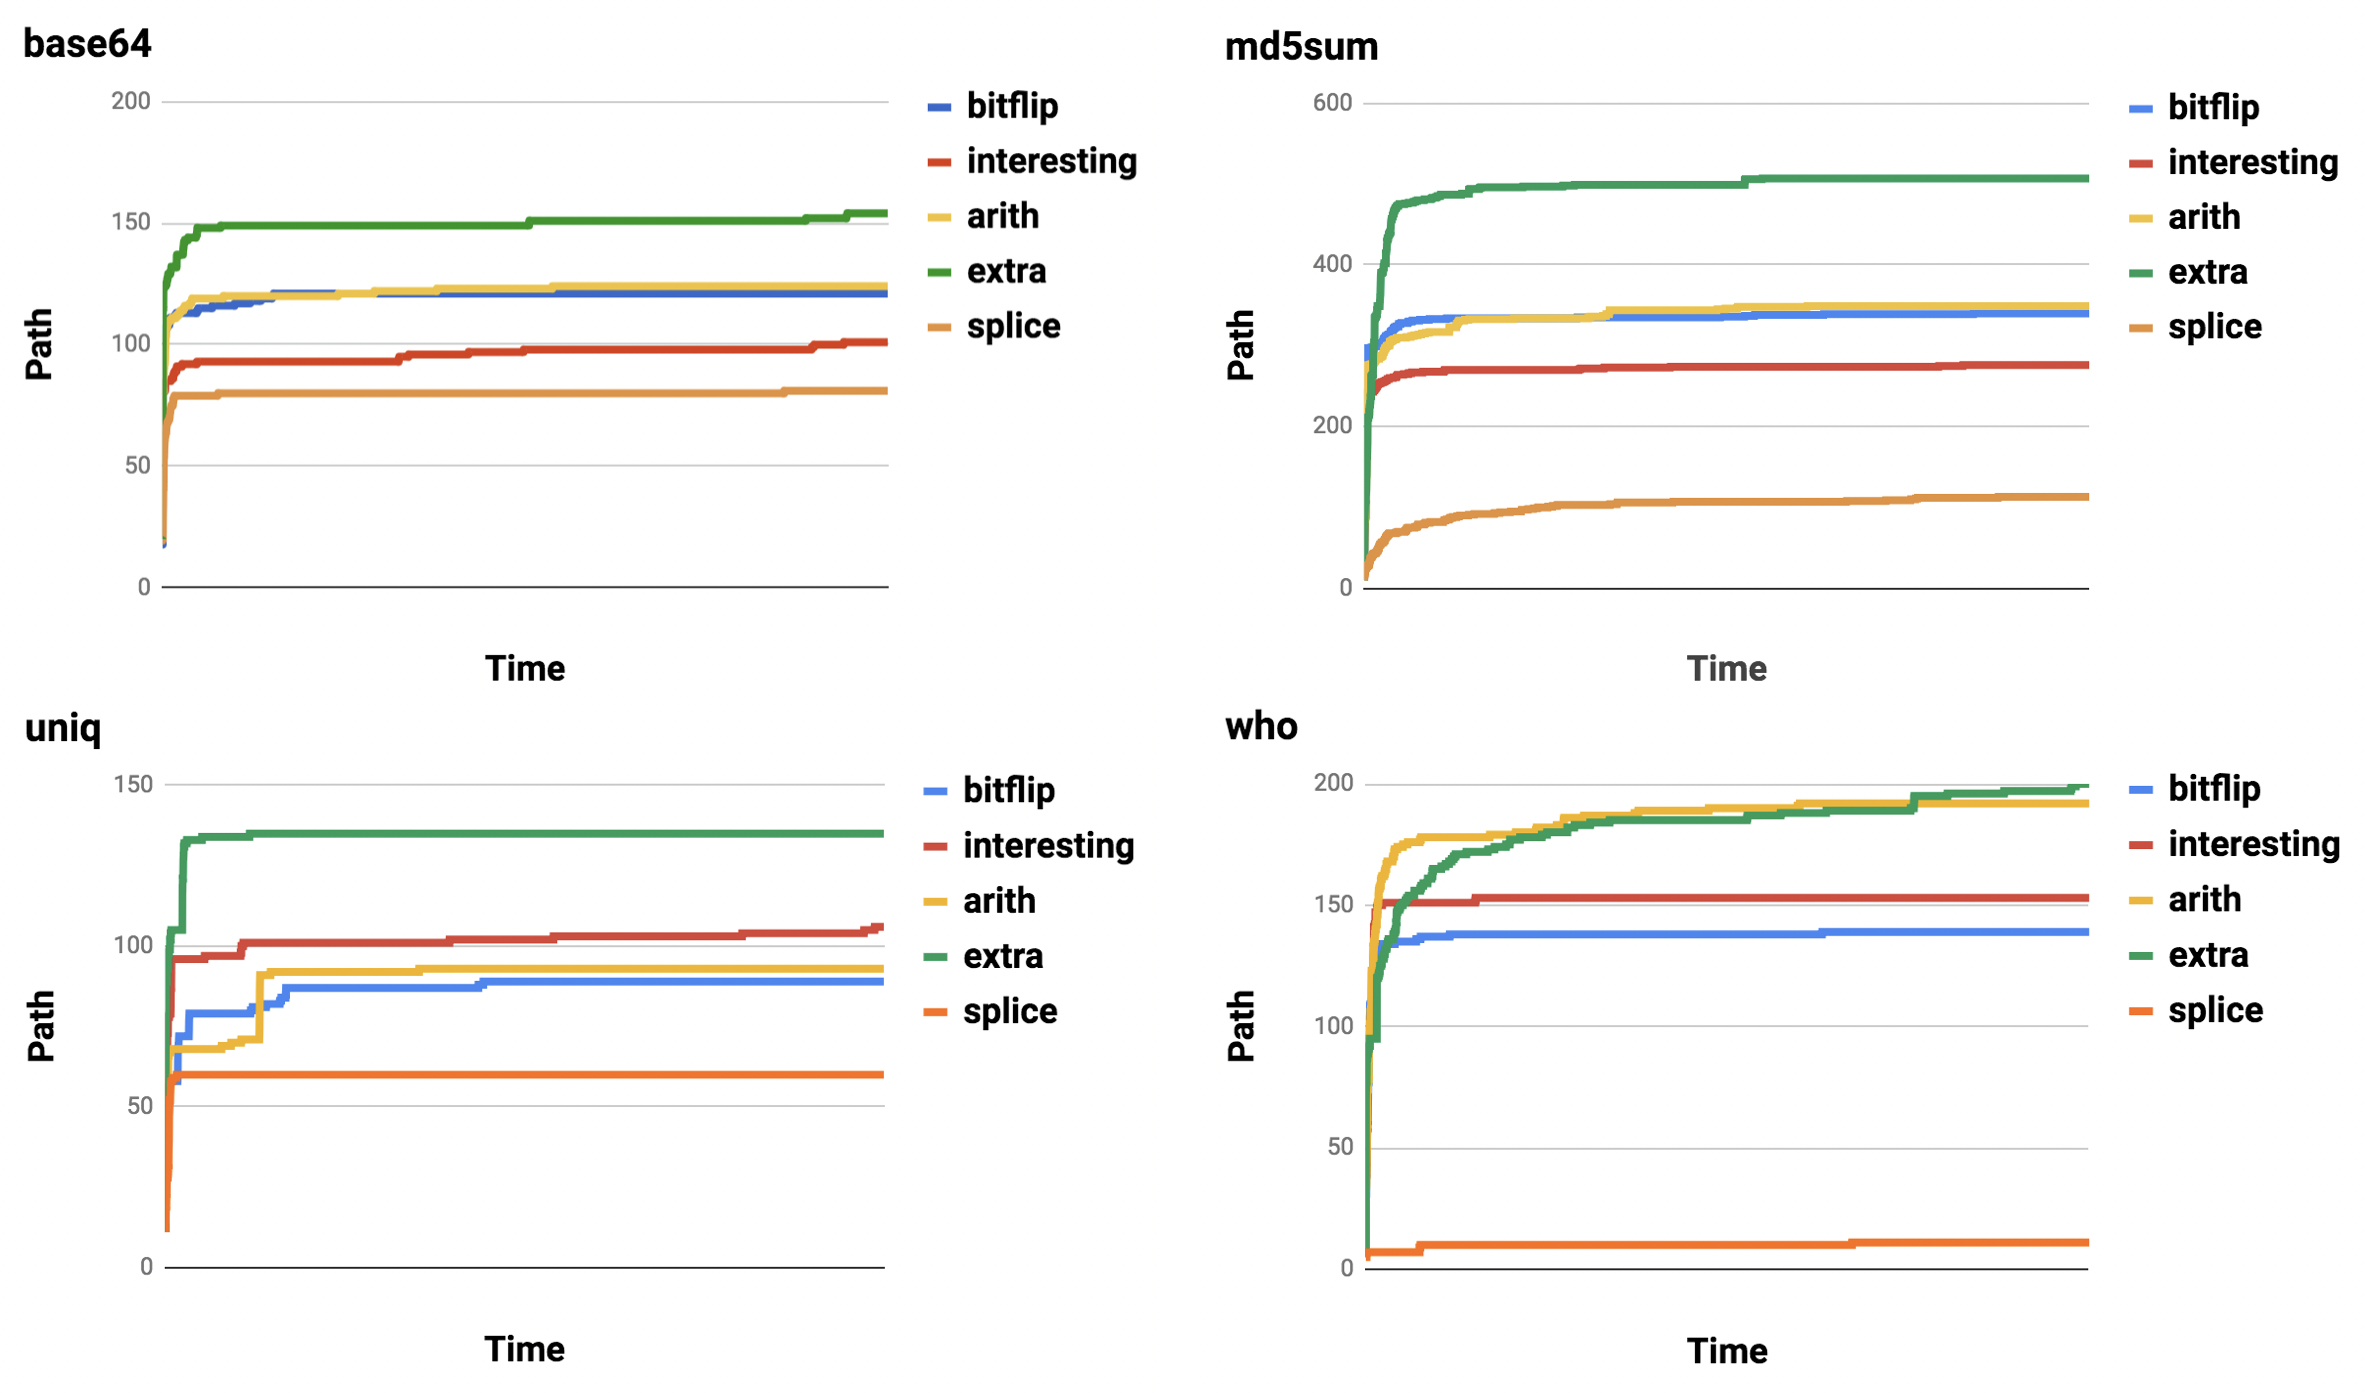
\includegraphics[width=3.6in]{pic/Mutators.png}
    \caption{Performance of Different Mutators }
    \label{Mutators}
\end{figure}

Thus, an empirical evaluation of AFL's five mainstream kinds of mutators is performed to answer above question. The statistical result on LAVA-M data set is shown in Fig.\ref{Mutators}. It indicates that (1) different kinds of mutation operators have different power for path growth; (2) extra (i.e., block-level deletion, insert and overwrite) mutation operators have better performance to help path growth, while splice mutation operators perform poor in general.

Motivated by above observation, granularity-aware scheduling of mutators is proposed. The proportion of mutation operators, which has better ability to trigger new paths (e.g., extra mutators) will be increased gradually. And over time, number of mutation operators that are chosen to applied on the seed is increased too. More specific, the scheduling algorithm for mutation operators is illustrated in algorithm \ref{schedule}.

\begin{algorithm}[h]
\caption{MutateInput(): Schedule of Mutators} 
\label{schedule}
\hspace*{\algorithmicindent} \textbf{Input}:  $s$, the seed to be mutated. \\
\hspace*{\algorithmicindent} \textbf{Input}:  $i$, the number of generated new test case.\\
\hspace*{\algorithmicindent} \textbf{Output}: $t$, the generated new test case.

\begin{algorithmic}[1]
        \STATE $\beta$= 1/ 3$^{process\_time}$;
        \STATE $p \leftarrow iteratorNum(i) * (1 -\beta)$
        \STATE $s' \leftarrow$ \texttt{RandomMutate}($s$, $p*(1-\alpha + \beta)$);
        \STATE $t \leftarrow$ \texttt{ExtraMutate}($s'$, $p * (\alpha - \beta$));
        \STATE return $t$
\end{algorithmic}
\end{algorithm}

Where $p$ represents number of selecting and applying different granularity mutation operators. The $process\_time$ refers to the execution time of fuzzing. And $\alpha$ is a constant ratio to conduct extra mutation. Over time, the $\beta$ will become smaller, and proportion of extra mutators will become higher. At the same time, $p$ becomes bigger,  and modification will become more full. In practice implementation, the $\alpha$ is set to 0.3.



